\paragraph{}
Sopra Steria est une entreprise de services du numérique devenue aujourd'hui le leader européen de la transformation numérique. Cette dernière accompagne les métiers dans leur transformation digitale en leur fournissant des services de conseils et en leur permettant d'établir les spécifications qui répondront au mieux à leurs attentes concernant la mise en place d'un système informatique. Elle assure ensuite toute la chaîne de production en réalisant la conception, le développement et la mise en production des solutions créées ainsi que leur maintien une fois ces dernières déployées.

\begin{figure}[h]
	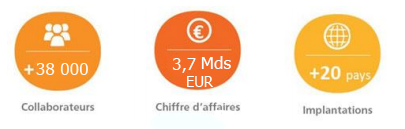
\includegraphics[scale=1]{images/sopraSteriaChiffres.png}
	\centering
	\caption{Quelques chiffres}
	\label{sopraSteriaChiffres}
\end{figure}

\paragraph{}
Elle compte plus de 38 000 collaborateurs présents dans plus de 20 pays différents et dispose d'un très grand nombre de savoir-faire informatiques qui lui permettent de d'offrir un panel de services extrèmement complet. Celle-ci est côtée en Bourse et réalise en 2016 un chiffre d'affaires de 3.7 milliards d'euros dont la majeure partie provient de ses actions réalisées en France et au Royaume-Uni.

\begin{figure}[h]
	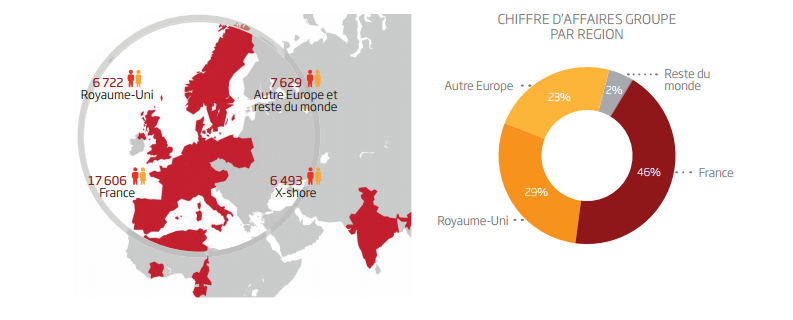
\includegraphics[scale=0.9]{images/sopraSteriaMonde.png}
	\centering
	\caption{Répartition internationale}
	\label{sopraSteriaMonde}
\end{figure}
		
		